%!TEX root = ../master_thesis.tex

\chapter{Constructing qualitative fault trees}
\label{chapter:fault_trees}

In this chapter we describe how a dependency graph can be transformed into a qualitative fault tree. First we lay the basis for our algorithm by describing the requirements towards the dependency graph and assumptions regarding failure semantics of applications. We then describe our algorithm and finish the theory section by introducing related work. Furthermore we describe how we executed our algorithm in the context of the case study and end the chapter by discussing our findings and future work.

\section{Theory}

In this section we explain our algorithm to transform a dependency graph into a qualitative fault tree. A dependency graph is a graph representing applications as vertices and dependencies between these applications as directed edges (see earlier \nref{chapter:dependency_graph}). The algorithm has several assumptions which we will describe before we explain the algorithm itself.

\subsection{Dependency graph requirements}
\label{section:fault_tree_graph_req}

For our algorithm to work, the dependency graph has to fulfill the following requirements:

\begin{tdescription}
  \item[Directed graph] In a directed graph, all edges have a direction from a source vertex to a destination vertex. In a dependency graph, all edges fulfill this property, since dependencies between applications are directed. If this requirements is not fulfilled, our algorithm could not construct a fault tree, since it would be impossible to detect the direction of failure propagation. Interpreting undirected edges as symmetric (being directed in both directions) is not a feasible solution, since the graph needs to be acyclic, as explained next.
  \item[Acyclic graph] An acyclic graph is a directed graph which has no cycles. This means that for every vertex, if one recursively follows the outgoing edges, one will never return to the start vertex. Fulfilling this requirement in a dependency graph might be hard, since service dependencies can be cyclic. If this requirement is not fulfilled, it will not be possible to generate a fault tree with our algorithm, since the generated tree will grow indefinitely.
    \item[Rooted graph] In a rooted graph, one vertex is labeled as a special vertex, distinguishing it from others. In our case, this can be fulfilled by manually choosing a root vertex from the graph. If this requirement is not met, it is not possible to identify the vertex for the TOP event for the fault tree and therefore the algorithm can not be executed. Given a microservice architecture that implements a SaaS, interesting root vertices are applications that directly serve clients, since these represent entry points into the system.
\end{tdescription}

When executing the algorithm, it will practically be executed on a subgraph of the dependency graph, which includes all vertices and edges reached when recursively following the outgoing edges from the root vertex. It is sufficient if only that subgraph is directed and acyclic.

\subsection{Failure semantics}
\label{s:failure_semantics}

In this section we describe the assumptions about failure semantics that we base our algorithm for fault tree construction on. In short, these are as follows: 1. Applications might fail because of \textbf{internal} failures. 2. The failure of one application might \textbf{propagate} failure to all applications that depend on it. Next we will describe these assumptions in more detail.

Given that we have a dependency graph, each vertex represents one application that is part of the microservice architecture. These applications might fail individually\footnote{To be correct with the terminology from the earlier \nref{subsec:dependability_threats}, it should be ``might individually be in erroneous states, which manifest as failure events when the service is used''. For reasons of comprehensibility, we only use the terms ``fail'' and ``failure'' to refer to these cases in this section.}.

In order to exhibit a failure, the application needs to have experienced a fault. We assume that there are only two possible fault types:
\begin{tenumerate}
  \item An application might experience an \emph{internal fault}. We specify that this fault might not be because of another application's failure. Apart from that, the nature of these internal faults it not specified more here\footnote{Examples for internal faults might be design or programming mistakes when considering the application itself or failures of the execution environment. We do not consider these internal faults further in our algorithm. As future work, these could be investigated further. For example, they could be modeled with own fault trees then.}.
  \item An application might experience an \emph{external fault}. A external fault in an application A occurs, when an application B has a failure and application A has a service dependency on application B.
\end{tenumerate}

The second fault type is based on service dependencies. We defined service dependencies in earlier \nref{sec:software_environment_terminology} as the fact that application A is the service consumer of another application B, which in turn is based on the fact that one process of application A at runtime opens a network connection to a service implemented by application B.

On a more abstract note, a dependency is defined by Knight~\cite{FundamentalsDepComputing} as following: ``The dependency of system A on system B represents the extent to which system A's dependability is (or would be) affected by that of system B''. In our case we assume that the dependence between systems is very strong, leading to the immediate propagation of failures.

In practice, the dependence might not be as strong as we assume it here. Commonly fault tolerance means are used to limit the impact of dependency failures. In our concrete example this might include using spatial or temporal redundancy, or continuing in a degraded state, with some functionality of the application being disabled but others being unaffected. We explicitly do not include these means of fault tolerance in our model of failure semantics.

The practical manifestation of failures is not of concern a here. Following the failure semantic model for distributed system by Cristian~\cite{cristian}, failures could be response, timing, omission or crash failures. All result in the same failure propagation results as proposed here.

% Assumption: two failure semantics: omission failure (detected by client via timeout) or crash failure (detected by client with error response from server). In both cases it is assumed that the application does not fullfil its purpose, thus the service consumer's dependency to this application is broken. \ref{ss:failure semantics}

\subsection{Construction algorithm}
\label{subsec:fault_tree_construction}

We introduced fault trees in \nref{subsec:theory_faulttree} as a technique for structured dependability analysis. Via a graphical diagram it helps to visualize which events may contribute to a TOP event failure and how these are interrelated with each other. We described earlier that fault trees are used to comprehensively describe the causes for a TOP event failure. In this work, we limit the fault tree analysis to \emph{internal} faults in an application and \emph{propagated} faults due to failing service dependencies.

\paragraph{Algorithm}

Given that we have a rooted, directed, acyclic graph, we may construct a qualitative fault tree with the following algorithm:

\begin{tenumerate}
  \item Turn root vertex into TOP event
  \item Create OR-gate and connect it to TOP event
  \item Create basic event with name of root vertex and connect it to OR-gate
  \item Follow each outgoing edge of the \emph{current} vertex (beginning with root vertex) to the \emph{next} vertex
  \begin{tenumerate}
    \item Create intermediate event with next vertex name and connect it to OR-gate of the current vertex
    \item Create OR-gate and connect it to intermediate event
    \item Create basic event with next vertex name and connect it to OR-gate
    \item Repeat step 4 recursively for next vertex
  \end{tenumerate}
\end{tenumerate}

% \todo{introduce pruning here}

% \todo{example with three-tier web application, because everyone will be able to understand that instead of abstract example}

Figure~\ref{fig:fault_tree_graph_example} shows an example dependency graph. Vertex ``A'' is the root vertex. Figure~\ref{fig:fault_tree_graph_example_algorithm} shows each algorithm step while generating the fault tree. Since vertex ``A'' only has one outgoing edge, algorithm step 4 is executed only once for vertex ``B''. If vertex ``A'' would have more outgoing edges, algorithm step 4 would be executed for each of these. If vertex ``B'' would have outgoing edges, algorithm step 4 would be executed for each of these recursively.

It is to note that the dependency graph has the vertices ``D'' and ``E'', which we did not utilize in the algorithm execution. This is due to the fact that neither ``A'' nor ``B'' have outgoing edges to ``D'' or ``E''. Furthermore, ``D'' and ``E'' have symmetric edges and therefore form a circle. Since this does not meet our requirement of acyclicity, it is not possible to use our algorithm with them.

\begin{figure}[h]
  \centering
  \fbox{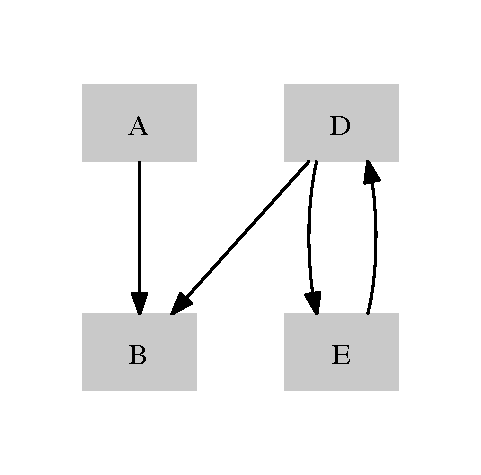
\includegraphics[width=0.4\linewidth] {images/qualitative-example/qualitative-fault-tree-example.pdf}}
  \caption{Example dependency graph for fault tree algorithm example. Root vertex is vertex ``A''.}
  \label{fig:fault_tree_graph_example}
\end{figure}

\begin{figure}[p]
  \centering
  \fbox{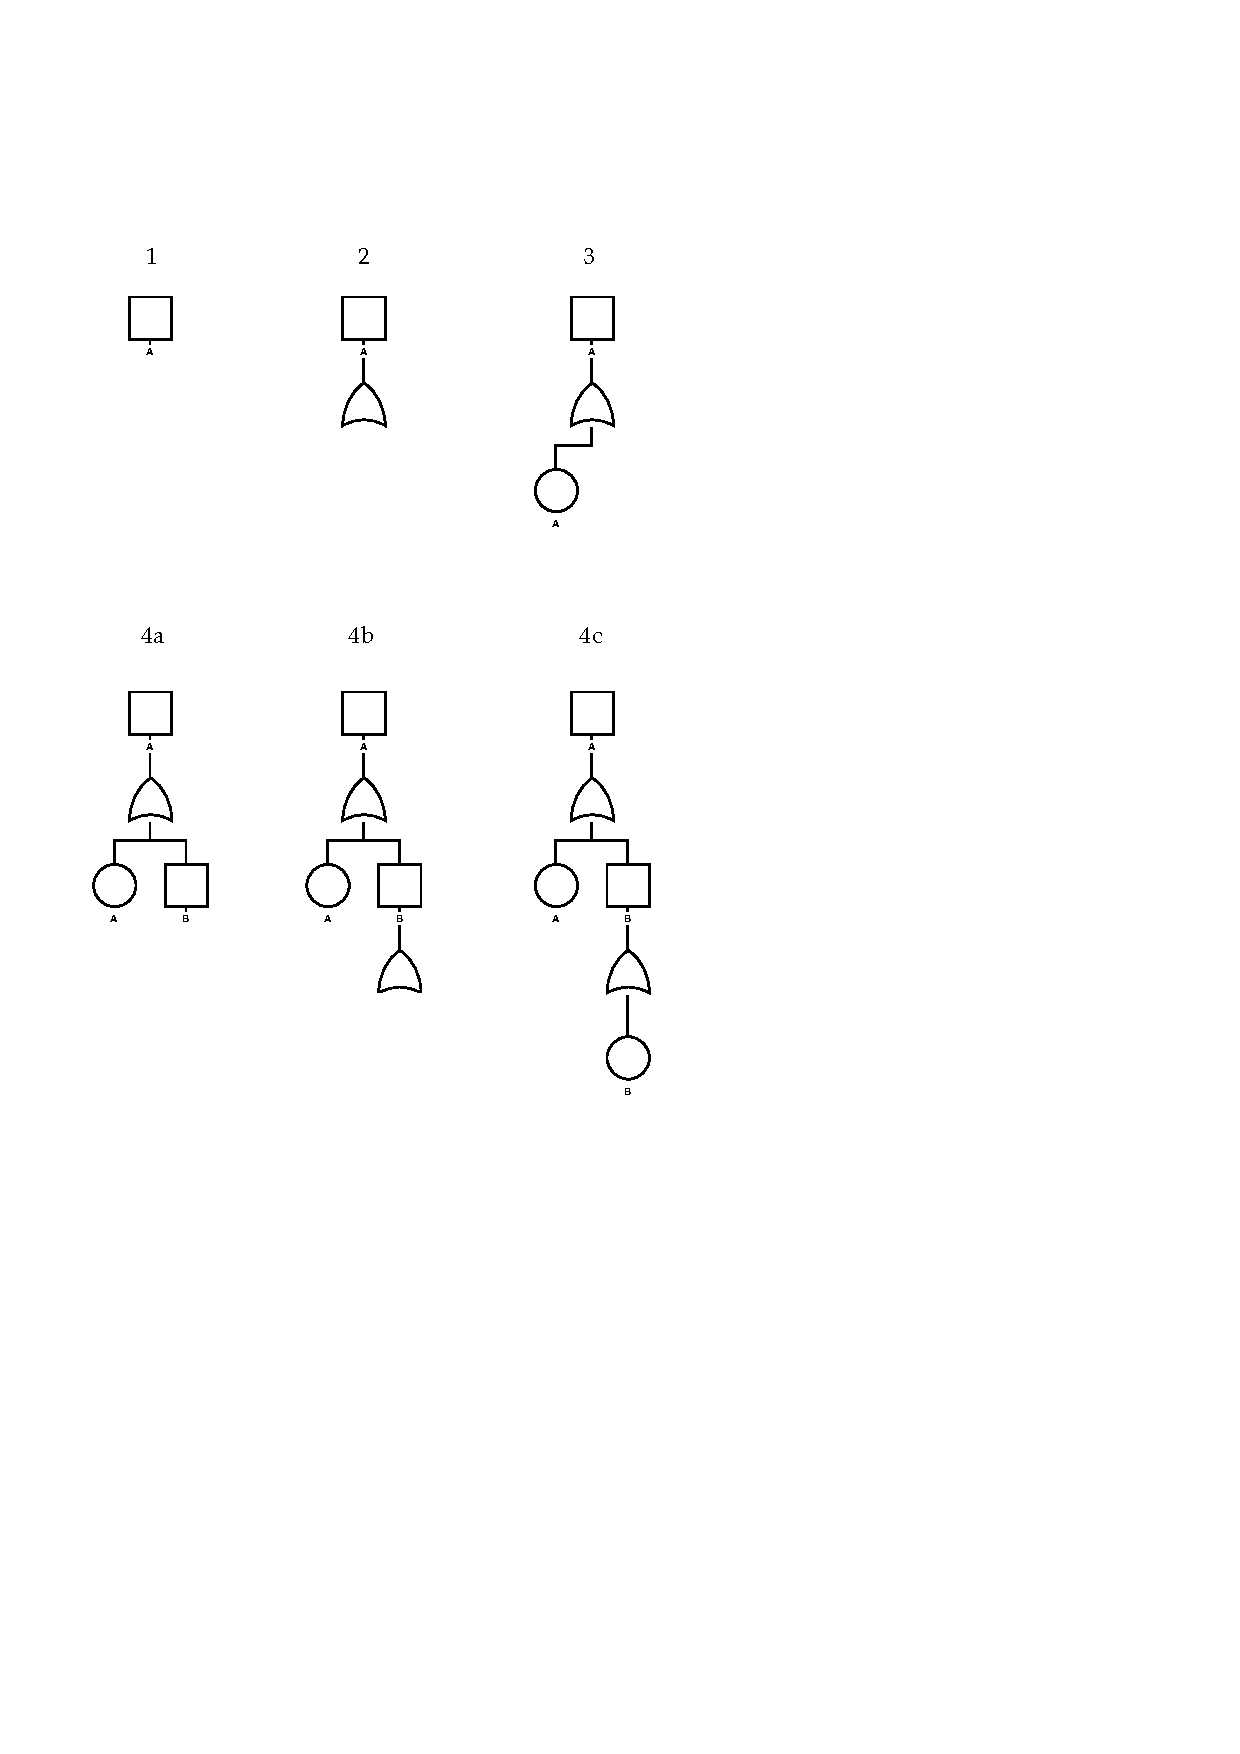
\includegraphics[width=0.9\linewidth] {images/qualitative-example/example-cropped.pdf}}
  \caption{Visualization of the algorithm for transforming a dependency graph to a qualitative fault tree. This example is based on the dependency graph in \autoref{fig:fault_tree_graph_example}}
  \label{fig:fault_tree_graph_example_algorithm}
\end{figure}

% \todo{include pruning into graph?}

\subsection{Related work}

Software fault tree analysis after Leveson et al. \cite{LevesonSoftwareFaultTrees} and Rausand et al \cite{SysReliabilityTheory} (section 4.3.8) is a software verification technique. It takes some undesired output of software as TOP event and then based on the internal structure of the software tries to derive if and how this output might occur. We do not use this technique in our work, since in our fault tree analysis we are not concerned with the internal structure of software but rather the system's view between software applications.

Lapp and Powers \cite{LAP77} proposed an algorithm for transforming directed graphs to fault trees that is similar to the one we propose here. It differs by taking more qualifying information into consideration and therefore constructing more expressive fault trees.

\section{Case study execution}
\label{sec:case_study_execution}

In this section we describe how we executed the algorithm in our case study. As basis for this we use the dependency graph in Figure \ref{fig:manual_annotation_whole} generated in \nref{subsec:graph_manual_annotation}. From that dependency graph, we chose two
root vertices to construct fault trees from: Vertex ``26'' and vertex ``73''.

% \todo{Can I rename these vertices to semantic names?}

\paragraph{Vertex ``26''} This vertex represents an application that acts as interface between the microservice architecture and the clients of the platform. Specifically, this application implements an API with the HTTP protocol, which is then used by the users' web browsers for functionality on the website \emph{\url{http://soundcloud.com}}. Therefore it does not have incoming edges, since clients (in this case browsers) are not represented in our investigation\footnote{see earlier \nref{sec:architecture} for more details}. When looking at the relevant subgraph spanning from vertex ``26'', it can be seen that there are cycles in that subgraph, revolving around vertex ``5''. We will comment in the \emph{evaluation} paragraph below on why these exist. To resolve this issue, we manually determined, which of the cyclic edges was more relevant, and removed the other edge. Figure \ref{fig:fault_tree_v2} shows the resulting fault tree for this root vertex. Please note that the fault tree is cropped, due to limitations with drawing large fault trees in the fault tree construction software we used. For reference and evaluation, Table \ref{tab:qualitative_size_comparison} shows statistics over the size of the fault tree with comparison to the size of the dependency graph it was based on. A second note is that for technical reasons the naming of the vertices in \autoref{fig:manual_annotation_whole} does not coincide with the naming of events in \autoref{fig:fault_tree_v2}.

% https://fuzzed.org/editor/932
% /Users/johan/Code/go/src/github.com/freenerd/thesis-tools/fuzzed/arch-all-masked-v2.graphml
\afterpage{%
\thispagestyle{empty}
  \begin{figure}[t]
    \vspace*{-0.9cm}
    \centering
    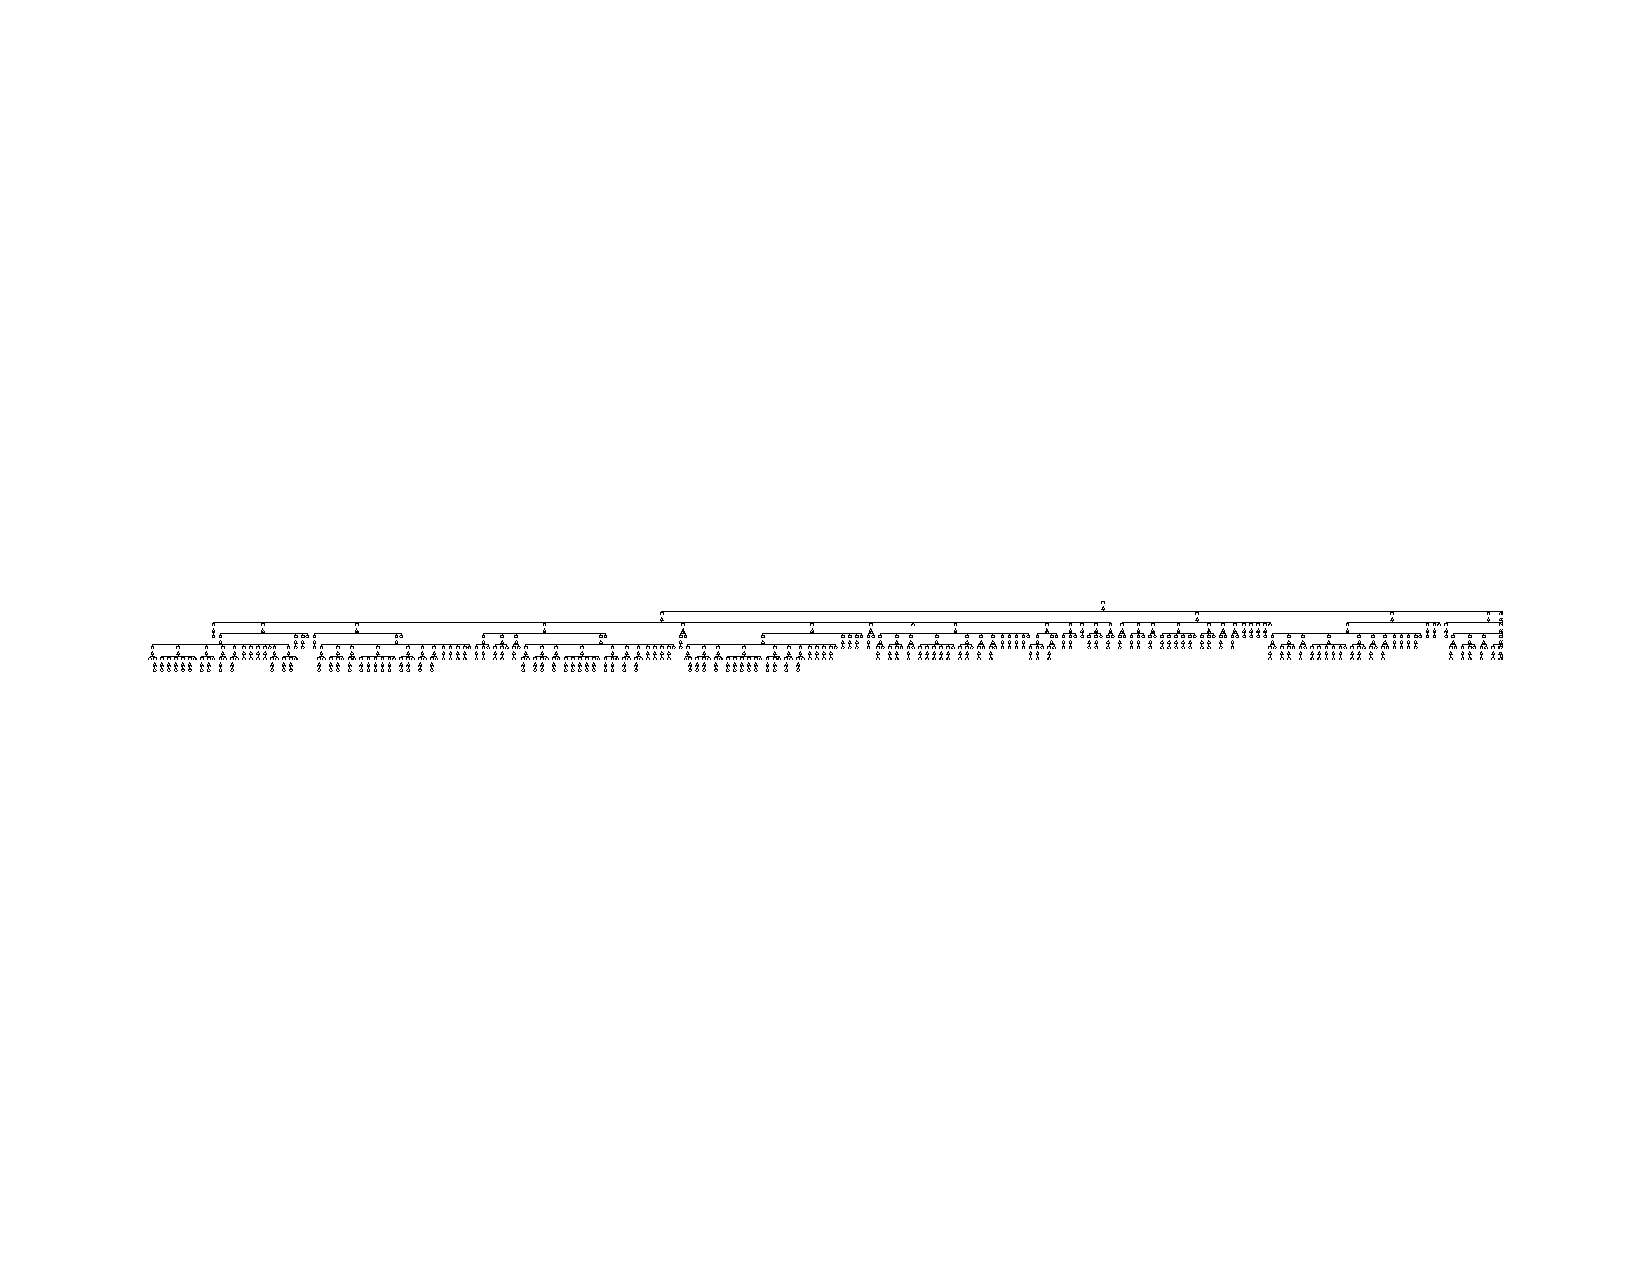
\includegraphics[angle=90, width=0.14\linewidth] {images/qualitative-fault-tree-v2-cropped.pdf}
    \caption{Qualitative fault tree for vertex ``26'' from case study dependency graph figure \autoref{fig:manual_annotation_whole} (cropped)}
    \label{fig:fault_tree_v2}
  \end{figure}
\clearpage
}

\paragraph{Vertex ``73'' (threaded-comments)} Similar to previous vertex ``26'', vertex ``73'' represents an application that exposes an API with the HTTP protocol to users' internet browsers. Therefore its vertex does not have incoming edges in our microservice architecture. We chose this vertex because we were interested in using a small subgraph for investigations in the following \nref{chap:quantitive_fault_tree}. For better visibility, we visualized the subgraph for vertex ``73'' in \autoref{fig:dep_graph_threaded_comments}. The vertices of the subgraph carry the original unmasked application identifiers as were assigned in \nref{subsec:graph_manual_annotation}. When extracting this subgraph, we made one major simplification: We did not include the outgoing edges for the vertex ``5'' in the dependency graph respectively application ``github.com/soundcloud/soundcloud'' in the subgraph. Our intention was to keep the subgraph small, in order to allow for further investigation in \nref{chap:quantitive_fault_tree}. We were not able to find another suitable subgraph which would allow these investigations without making the simplification we did here. The fault tree resulting from executing our algorithm on the subgraph can be seen in \autoref{fig:fault_tree_threaded_comments}.

\begin{figure}[h!]
  \centering
  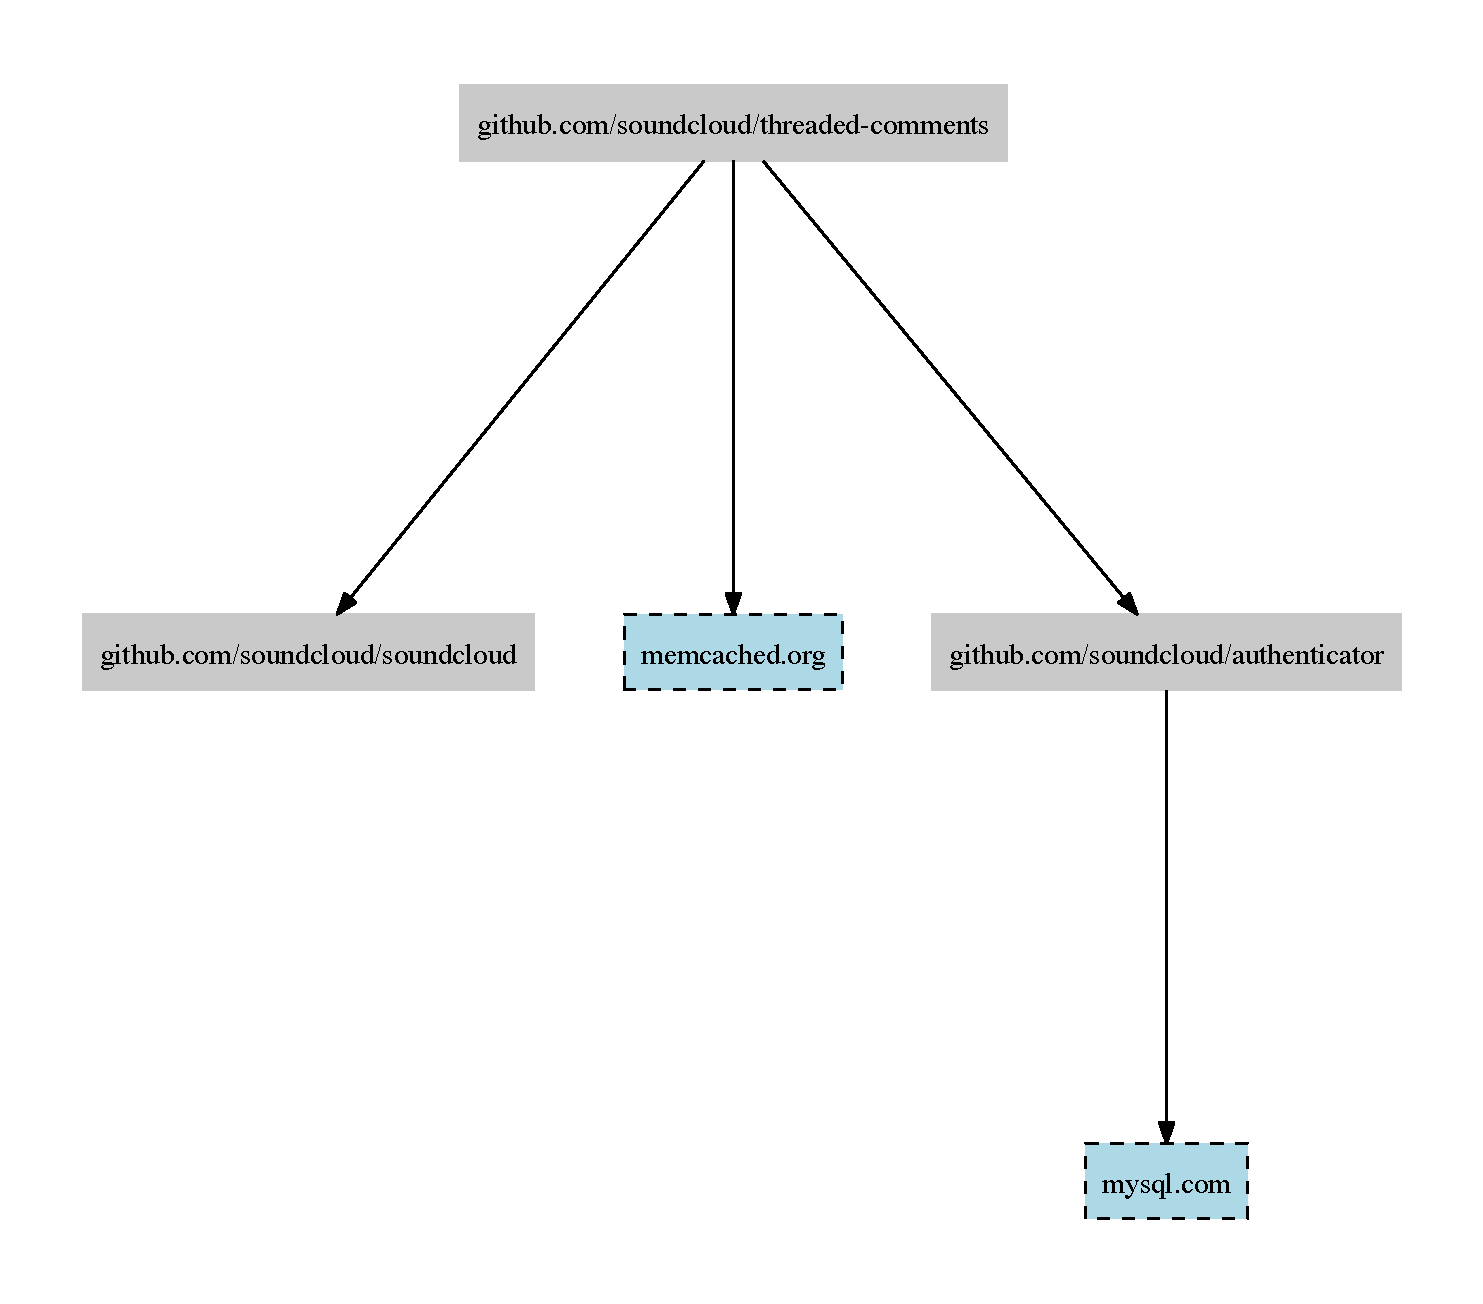
\includegraphics[width=0.6\linewidth] {images/dependencies-threaded-comments.pdf}
  \caption{Subgraph for vertex ``73'' from case study figure \autoref{fig:manual_annotation_whole}. The outgoing edges for vertex ``5''/application ``github.com/soundcloud/soundcloud'' have been removed. The vertex names have been unmasked to carry their original application identifiers.}
  \label{fig:dep_graph_threaded_comments}
\end{figure}

\begin{figure}[h!]
  \centering
  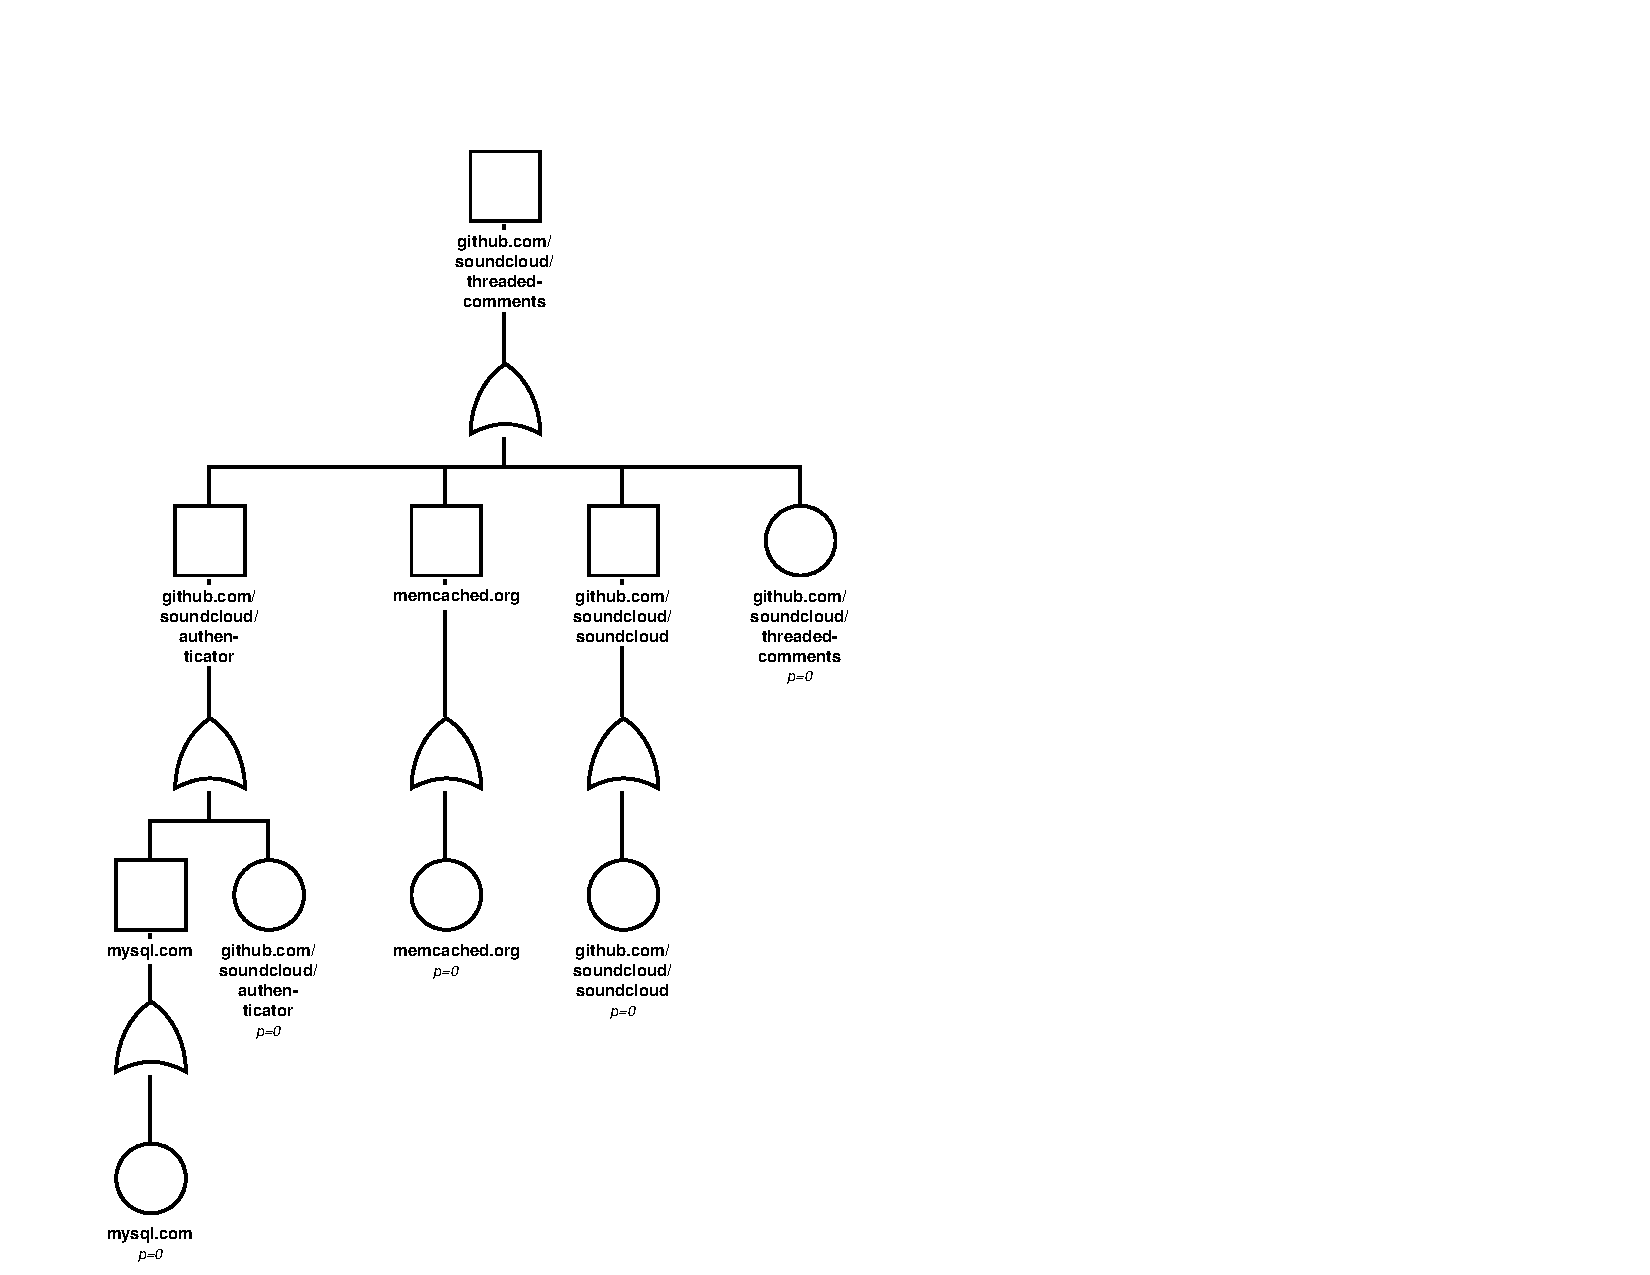
\includegraphics[width=0.6\linewidth] {images/threaded-comments-fault-tree-cropped.pdf}
  \caption{Qualitative fault tree for vertex ``73''/application ``github.com/soundcloud/soundcloud'' following the dependency graph from \autoref{fig:dep_graph_threaded_comments}.}
  \label{fig:fault_tree_threaded_comments}
\end{figure}

Please note that for brevity in this work, we have shortened the application identifiers as shown in \autoref{tab:shortened_app_names}. Furthermore, \autoref{tab:app_name_descriptions} shows descriptions for the applications involved.

\begin{table}
  \caption{Shortened application identifiers of subgraph for vertex ``73'' shown in \autoref{fig:dep_graph_threaded_comments}.}
  \label{tab:shortened_app_names}
  \begin{tabular}{ |l|l| }
    \hline
    Full application identifier & Shortened application identifier \\
    \hline
    github.com/soundcloud/soundcloud & soundcloud \\
    github.com/soundcloud/threaded-comments & threaded-comments \\
    github.com/soundcloud/authenticator & authenticator \\
    mysql.com & mysql \\
    memcached.org & memcached \\
    \hline
  \end{tabular}
\end{table}

\begin{table}
  \caption{Description of applications of subgraph for vertex ``73'' shown in \autoref{fig:dep_graph_threaded_comments}.}
  \label{tab:app_name_descriptions}
  \begin{tabular}{ |l|l| }
    \hline
    Shortened application identifier & Description\\
    \hline
    soundcloud & Former-monolithic main business logic application \\
    threaded-comments & Application to group and cache comments \\
    authenticator & Authentication and authorization of requests \\
    mysql & Relational database \\
    memcached & In-memory key-value, used as cache store \\
    \hline
  \end{tabular}
\end{table}

\section{Discussion}

As we have seen with \autoref{fig:manual_annotation_whole} and \autoref{fig:dep_graph_threaded_comments}, it is possible to generate fault trees from dependency graphs with our algorithm. In this section we will discuss these and the algorithms.

The most notable fact of our algorithm is that it only uses OR-gates as logic gates. This leads to the fact that each basic event is a minimal cut set and therefore each basic event is a ``single point of failure'' for the TOP event. As a result of this fact, employing analytical methods that are based on cut set analysis will yield low insights. We believe that the architecture of the system is not holistically expressed in the generated fault tree, since all basic events have the exact same influence on the TOP event. As major reason for that structure we see the exclusion of fault tolerance in the construction process. We will discuss opportunities for including these during automatic execution in the following future work section.

Table \ref{tab:qualitative_size_comparison} shows the sizes of the dependency graphs and the fault trees that our algorithm generated for them. It can be seen that the fault trees have magnitudes more elements and edges than the dependency graphs. One reason for the size increase is the duplication of dependency subgraphs in the fault tree: If a vertex has several incoming edges, the subgraph spanned by its outgoing edges will be present several times in the fault tree, since it will be duplicated for each incoming edge. Another reason for the size increase is the usage of intermediate events and logic gates, which are not necessary in the dependency graph.

% ~GOPATH/src/github.com/freenerd/thesis-tools/graphs/cat arch-all-masked.dot (look for biggest number)
% ~GOPATH/src/github.com/freenerd/thesis-tools/graphs/cat arch-all-masked.dot | grep "\->" | wc

% cat ~GOPATH/src/github.com/freenerd/thesis-tools/fuzzed/arch-all-masked-v2.graphml | grep edge | wc
% ~GOPATH/src/github.com/freenerd/thesis-tools/fuzzed/cat arch-all-masked-v2.graphml | grep "basicEvent" | wc
%

One of the assumptions of our algorithm is that there are no circles in the graph. As we have seen in the case study, circles do appear in reality, which hinders using the algorithm. We manually resolved the dependencies in the case study, which we believe is a poor solution.

We believe that for an engineer to get an overview over the architecture, dependency graphs are better suited than fault trees, due to their significantly smaller size. We see potential in improving the algorithm as explained in the following Future work section. We also see potential of the fault trees as basis for quantitative fault trees, as explained in the following \nref{chap:quantitive_fault_tree}.

\vfill\clearpage

\begin{table}[!ht]
  \caption{Sizes of dependency graphs and the generated fault trees}
  \label{tab:qualitative_size_comparison}
  \begin{tabular}{ |l|l| }
    \hline
    \multicolumn{2}{|l|}{Dependency graph with root vertex ``26'' (not visualized)} \\
    Vertices & 49 \\
    Edges & 97 \\
    \hline
    \multicolumn{2}{|l|}{Fault tree for vertex ``26'' \autoref{fig:manual_annotation_whole}} \\
    Elements & 1146 \\
    Basic Events & 382 \\
    Edges & 1145 \\
    \hline
    \multicolumn{2}{|l|}{Dependency graph with root vertex ``73'' \autoref{fig:dep_graph_threaded_comments}} \\
    Vertices & 5 \\
    Edges & 4 \\
    \hline
    \multicolumn{2}{|l|}{Fault tree for vertex ``73'' \autoref{fig:manual_annotation_whole}} \\
    Elements & 15 \\
    Basic Events & 5 \\
    Edges & 14 \\
    \hline
  \end{tabular}
\end{table}

% On the bottom are backing applications. They provide a service, but don't consume one themselves. Typical examples are data storage systems.

\section{Future work}

In the discussion we have seen that the size of the fault tree is problematic. We see two opportunities for future work to improve on that:
\begin{titemize}
  \item To reduce the number of elements and edges in the fault tree, we see the following simplification: All vertices with no outgoing edges will follow the same pattern of being represented by one intermediate event, one OR-gate and one basic event. These can be compacted by removing the intermediate event and OR-gate, and connecting the basic event directly to the parent OR-gate.
  \item We have discussed that the same subgraph may appear several times in the fault tree. To improve on that, a ``Transfer In'' element\footnote{A ``Transfer In'' element is a fault tree element that allows to include another fault tree. The ``Transfer In'' element then represents the TOP event of the included fault tree.} may be used.
\end{titemize}

The fault trees our algorithm generated are limited to OR-gates as logic gates only. This limits the applicability of analytical methods based on cut sets. Thus the goal of future work should be to improve the expressiveness of the fault tree. Next we will introduce several opportunities for that:
\begin{tdescription}
  \item[Manual extension] The generated fault tree could be taken as a basis for manual extension by engineers. Examples for extensions are including runtime environments of applications, non-technical influences like human interaction, or the methods introduced below.
    \item[Application fault tolerance] Future work should investigate representing fault tolerance of applications in the fault trees. Examples for application-internal fault tolerance mechanisms to investigate are temporal and spatial redundancies (which might result in using AND-gates or K/N-gates in the fault tree) as well as degraded service (which might allow for splitting applications into finer-grained functionalities).
    \item[Different application granularity] In earlier \nref{section:graph_future_work} for generating dependency graphs, we already discussed potential for different granularities for applications. These might be deploys, processes or functionality. Each of these would allow different algorithms, which in turn would result in different fault trees. These could aid the expressiveness of the fault tree.
    \item[Infrastructure applications] In our investigations, we did not take infrastructure applications (like deployment systems or traffic management systems) into consideration. Future work could investigate how to include these in the algorithm. This would improve the scope of the fault tree in the direction of a more holistic view. It might also help to model system fault tolerance, since it is sometimes realized through infrastructure applications (e.g. load balancers).
\end{tdescription}

\section{Summary}

In this chapter we suggest qualitative fault trees as a way of modeling failure propagation in microservice architectures. We proposed a novel algorithm for transforming dependency graphs into qualitative fault trees. The algorithm respects two kinds of failures: internal failures from applications themselves and external failures propagating through the architecture via service dependency failures. Fault tolerance mechanisms were not considered. We executed the algorithm for one application of the case study's dependency graph with the resulting qualitative fault tree visible in \ref{fig:fault_tree_threaded_comments}.